%!TEX root = ../Demo.tex
\chapter{引言}
视频监控技术的发展,给人们的生活和生产带来了极大的便利和充分的安全保障。
视频监控系统是安防领域中的研究热点,随着近年来各类智能设备数量的爆发性增长,视频监控系统正朝着数字化、智能化、网络化、人性化的方向发展。
随着人们生活水平的提高,人们更多的把目光投向了如何更好的保护自己和家人的人身安全以及经济财产,因此以前只出现在公共场所的监控摄像头,如今在人们的家中就能看到它们的身影,希望通过它们可以随时随地的对人或物进行安放监控。

视频实时监控系统是一个可以实时对远程监控摄像头采集的画面进行实时监测的平台。
Web端的视频实时监控系统可以依托手机、电脑等支持网页访问的设备进行查看,可以做到只要有网络,就可以随时随地查看监控视频。
传统的视频监控系统需要在一个局域网内,在一台终端机器上才能实现监控视频的查看。
本文提出了一种基于Spring Boot的视频实时监控系统的设计思路以及实现方法。

\chapter{关键技术}
本章将介绍系统开发设计过程中使用到的关键技术。

\section{流媒体传输技术}
实时的视频监控系统需要基于流媒体传输技术来实现,需要摄像头本身或者后置的图像处理服务器支持流媒体传输,常见的三种流媒体传输技术有:RTMP、HTTP-FLV和HLS。

\subsection{流媒体以及流式传输}
流媒体是指将一连串的媒体数据(包含音频、视频数据)压缩后,采用流式传输的方式发送数据,
在网上即时传输影音以供观赏的一种技术与过程,此技术使得数据包得以像流水一样发送;
如果不使用此技术,就必须在使用前下载整个媒体文件。
流媒体在播放前不会下载整个文件,只将开始部分存入内存,同时也会在用户访问时对数据包进行缓存,
让媒体数据正确地输出,流媒体数据流随时传送随时播放。

流式传输是指客户端通过链接流媒体服务器实时传输音频、视频数据,实现“边下载边播放”。
流式传输是实现流媒体的关键技术。
流式传输时,音频、视频等时基媒体由音视频服务器向用户计算机的连续、实时传送,
用户不必等到整个文件全部下载完毕,而只需经过几秒或十数秒的启动延时即可进行观看。
当音频、视频等时基媒体在客户机上播放时,文件的剩余部分将在后台从服务器内继续下载。
流式不仅使启动延时成十倍、百倍地缩短,而且不需要太大的缓存容量。
流式传输避免了用户必须等待整个文件全部从网络上下载才能观看的缺点。

% 在网络上传输音频、视频等多媒体信息,主要有下载和流式传输两种方案。
% 多媒体文件一般都较大,所以需要的存储容量也较大;
% 同时由于网络带宽的限制,通过下载实现的多媒体数据传输常常要花数分钟甚至数小时,
% 所以这种处理方法延迟也很大。

\subsection{基于RTMP的流媒体传输技术}
实时消息传输协议(即Real-Time Messaging Protocol,缩写RTMP) 最初是Macromedia公司为了满足在互联网上传输流媒体音视频而开发的一个私有协议。

RTMP(Real Time Messaging Protocol) 是由 Adobe 公司基于 Flash Player 播放器对应的音视频 flv 封装格式提出的一种,基于TCP 的数据传输协议。本身具有稳定、兼容性强、高穿透的特点。常被应用于流媒体直播、点播等场景。


\subsection{基于HTTP-FLV的流媒体传输技术}
\subsection{基于HLS的流媒体传输技术}

\section{Spring Boot开发框架}

\subsection{概述}
Spring Boot是由Pivotal团队提供的全新框架,其设计目的是用来简化新Spring应用的初始搭建以及开发过程。该框架使用了特定的方式来进行配置,从而使开发人员不再需要定义样板化的配置。

Spring Boot不仅继承了Spring框架原有的优秀特性,而且还通过简化配置来进一步简化了Spring应用的整个搭建和开发过程。
在Spring Boot出现之前,使用Spring框架进行应用开发需要编写繁琐的配置文件,然而这些配置文件的内容大多都是类似的。

\subsection{控制反转特性}
Spring框架具有控制反转(IOC)特性,IOC旨在方便项目维护和测试,它提供了一种通过Java的反射机制对Java对象进行统一的配置和管理的方法。

\subsection{面向切面编程}
Spring框架具有面向切面编程(AOP)框架,SpringAOP框架基于代理模式,同时运行时可配置;AOP框架主要针对模块之间的交叉关注点进行模块化。


\section{对象拷贝技术MapStruct}

\section{内存数据库Redis}

\section{RBAC权限系统}


\chapter{系统总体设计}

\section{数据库设计}

\section{实体关系设计}

\begin{figure}[ht]
    \centering
    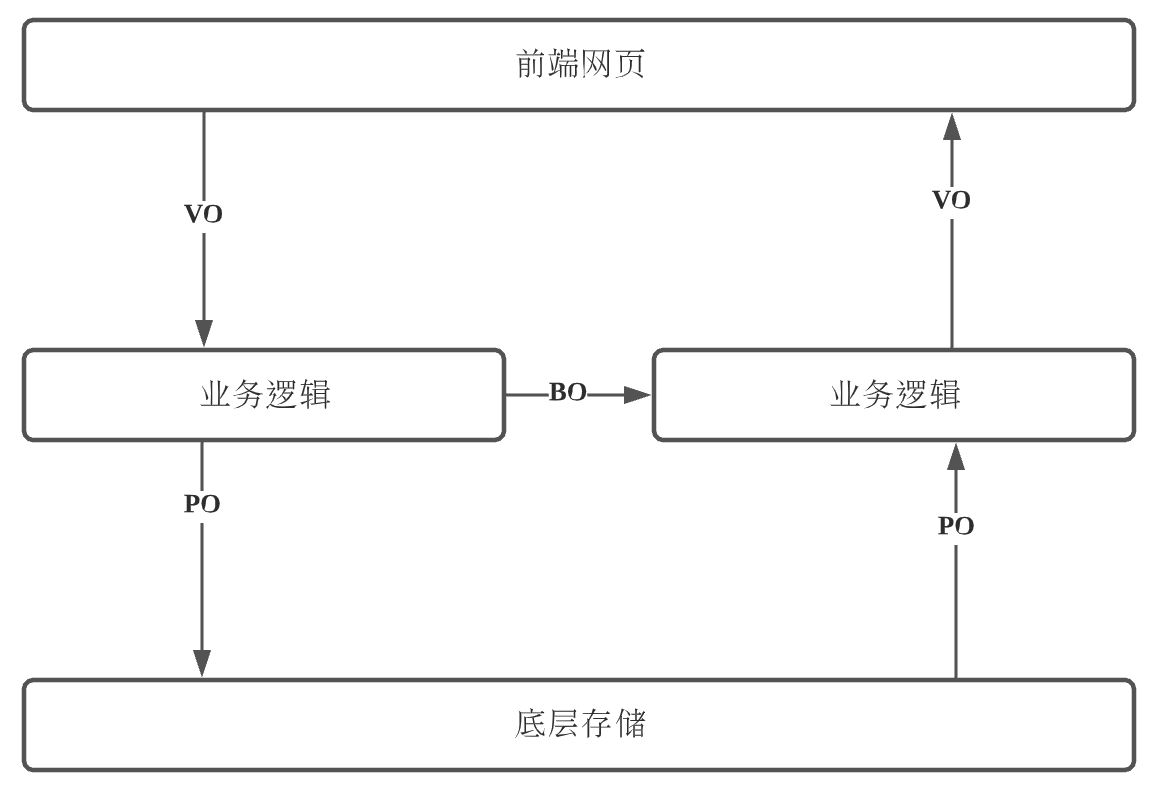
\includegraphics[width=0.8\linewidth]{./Figure/IMG_1.png}
    \caption{西电1}\label{Fig:xd1}
\end{figure}


























\chapter{系统实现}
